\documentclass[border=10pt]{standalone}
\usepackage{tikz}
\usepackage{amsmath}
\usepackage{graphicx}

\begin{document}

% -------------------------
% SQUARE GRID (Z^2)
% -------------------------
\resizebox{!}{6cm}{%
    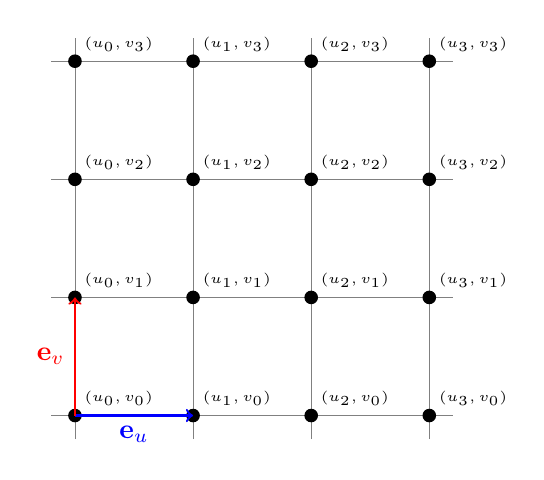
\begin{tikzpicture}[scale=1.5]
        \draw[step=1cm, gray, very thin] (-0.2,-0.2) grid (3.2,3.2);
        \foreach \u in {0,...,3} {
            \foreach \v in {0,...,3} {
                \filldraw[black] (\u,\v) circle (1.5pt);
                \node[above right, font=\tiny] at (\u,\v) {$(u_{\u},v_{\v})$};
            }
        }
        % Basis vectors
        \draw[->, thick, blue] (0,0) -- (1,0) node[midway, below] {$\mathbf{e}_u$};
        \draw[->, thick, red] (0,0) -- (0,1) node[midway, left] {$\mathbf{e}_v$};
    \end{tikzpicture}%
}
\hspace{1cm}
% -------------------------
% HEXAGON GRID (Corrected Axial Mapping)
% -------------------------
\resizebox{!}{6cm}{%
    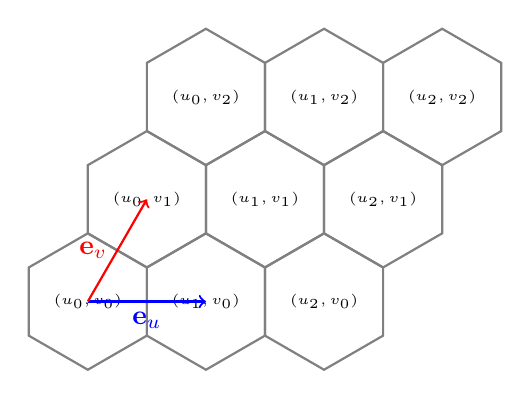
\begin{tikzpicture}[scale=1.5]
        % Circumradius R = 1/sqrt(3) guarantees the distance between adjacent centers is exactly 1
        \def\R{0.57735} 
        
        \foreach \u in {0,...,2} {
            \foreach \v in {0,...,2} {
                % Axial offset mapping: x = u + v/2, y = v * sqrt(3)/2
                \pgfmathsetmacro\x{\u + \v/2}
                \pgfmathsetmacro\y{\v * 0.866025}
                
                % Draw a flat-topped hexagon correctly centered using a coordinate shift
                \draw[gray, thick, shift={(\x,\y)}] 
                    (30:\R) -- (90:\R) -- (150:\R) -- 
                    (210:\R) -- (270:\R) -- (330:\R) -- cycle;
                    
                % Label the center coordinates
                \node[font=\tiny] at (\x,\y) {$(u_{\u},v_{\v})$};
            }
        }
        
        % Basis vectors
        \draw[->, thick, blue] (0,0) -- (1,0) node[midway, below] {$\mathbf{e}_u$};
        \draw[->, thick, red] (0,0) -- (0.5,0.866025) node[midway, left] {$\mathbf{e}_v$};
    \end{tikzpicture}%
}
\hspace{1cm}
% -------------------------
% TRIANGLE GRID (Sheared Bisection)
% -------------------------
\resizebox{!}{6cm}{%
    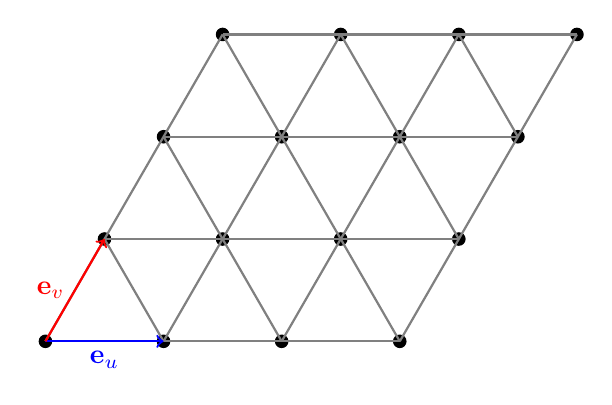
\begin{tikzpicture}[scale=1.5]
        % Draw Vertices
        \foreach \u in {0,...,3} {
            \foreach \v in {0,...,3} {
                \pgfmathsetmacro\x{\u + \v/2}
                \pgfmathsetmacro\y{\v * 0.866025}
                \filldraw[black] (\x,\y) circle (1.5pt);
            }
        }
        
        % 1. Draw horizontal edges (u to u+1)
        \foreach \v in {0,...,3} {
            \draw[gray, thick] (\v/2, \v*0.866025) -- (3 + \v/2, \v*0.866025);
        }
        
        % 2. Draw +60 degree edges (v to v+1)
        \foreach \u in {0,...,3} {
            \draw[gray, thick] (\u, 0) -- (\u + 1.5, 3*0.866025);
        }
        
        % 3. Draw -60 degree edges to bisect rhombi into Left and Right triangles
        \foreach \u in {0,...,2} {
            \foreach \v in {0,...,2} {
                \pgfmathsetmacro\xtop{\u + (\v+1)/2}
                \pgfmathsetmacro\ytop{(\v+1) * 0.866025}
                \pgfmathsetmacro\xbot{\u + 1 + \v/2}
                \pgfmathsetmacro\ybot{\v * 0.866025}
                \draw[gray, thick] (\xtop,\ytop) -- (\xbot,\ybot);
            }
        }
        % Basis vectors
        \draw[->, thick, blue] (0,0) -- (1,0) node[midway, below] {$\mathbf{e}_u$};
        \draw[->, thick, red] (0,0) -- (0.5,0.866025) node[midway, left] {$\mathbf{e}_v$};
    \end{tikzpicture}%
}

\end{document}